% !TEX program = xelatex
\documentclass[11pt, a4paper]{article}

\usepackage[top=2cm, bottom=2cm, left=2.5cm, right=2cm]{geometry}
\usepackage{fontspec}
\setmainfont{Times New Roman}
\setsansfont{Arial}
\setmonofont{Courier New}[Scale=0.95]
\usepackage{amsmath, amssymb}
\usepackage{booktabs}
\usepackage{tabularx}
\usepackage{graphicx}
\usepackage{float}
\usepackage{xcolor}
\usepackage{hyperref}
\usepackage{xurl}
\usepackage{parskip}
\usepackage{microtype}
\usepackage{caption}
\usepackage{subcaption}
\usepackage{enumitem}
\usepackage{fvextra}
\usepackage{tikz}
\usetikzlibrary{positioning, arrows.meta}

\graphicspath{{images/}}
\emergencystretch=10em

\hypersetup{
    colorlinks=true,
    linkcolor=blue!70!black,
    citecolor=blue!70!black,
    urlcolor=blue!70!black,
    pdftitle={Agent - AI Agents and Reinforcement Learning},
    pdfauthor={Nguyen Van Truong}
}

\DefineVerbatimEnvironment{codeblock}{Verbatim}{breaklines, breakanywhere, frame=single, framesep=2mm,
    fontsize=\small, rulecolor=\color{gray!60}}
\newcommand{\code}[1]{\texttt{#1}}
\setlist{itemsep=2pt, topsep=4pt}

\begin{document}

% ---------------------------------------------------------
% COVER PAGE
% ---------------------------------------------------------
\begin{titlepage}
\begin{center}

\vspace*{0.5cm}

\Large
\textbf{POSTS AND TELECOMMUNICATIONS INSTITUTE OF TECHNOLOGY}\\
\textbf{Faculty of Information Technology}

\vspace{2.0cm}

\Huge
\textbf{Intelligent System Development}\\
\vspace{0.4cm}
\LARGE
\textbf{AGENT}\\
\vspace{0.6cm}
\Large
\textbf{AI Agents and Reinforcement Learning:\\A Q-learning Agent in a Maze}

\vspace{1.2cm}

\vfill

\normalsize
\begin{tabular}{rl}
\textbf{Lecturer:} & Assoc. Prof. Dinh Que Tran, Ph.D. \\
\textbf{Email:} & quetd@ptit.edu.vn, tdque@yahoo.com \\[0.8cm]
\textbf{Student Name:} & Nguyễn Văn Trường \\
\textbf{Student ID:} & B23DCCE095 \\
\textbf{Semester:} & I.2025 -- 2026 \\
\textbf{Submission:} & Individual Project \\
\end{tabular}

\vfill

\textbf{Hanoi, 2026}

\vspace{0.5cm}

\end{center}
\end{titlepage}

{\small\tableofcontents}
\newpage

% =====================================================================
\section{Introduction}

A traditional program does exactly what its programmer wrote: \emph{if this happens, do that}. An \textbf{AI agent} is different. It is given a \emph{goal} and works out for itself which actions get it closer, adapting when the situation changes. One of the main ways an agent can learn which actions to choose is \textbf{reinforcement learning (RL)}: the agent tries actions, receives rewards or penalties, and gradually improves.

\textbf{The idea in one example.} Drop a robot at the corner of a maze and tell it only ``get to the opposite corner''. It is not told where the walls are. After every move it receives a score: a small penalty for each step, a big penalty for hitting a wall, a big prize for reaching the exit. At first it blunders around; after thousands of attempts it walks the shortest route. This report explains the ideas behind such an agent and then builds it.

The background in Sections~\ref{sec:agents}--\ref{sec:link} comes from two sources, listed in the references:

\begin{itemize}
    \item Google Cloud, \emph{``What are AI agents?''}, \url{https://cloud.google.com/discover/what-are-ai-agents}. It explains what an AI agent is, what it is made of, what types exist, and what agents are used for.
    \item GeeksforGeeks, \emph{``What is Reinforcement Learning?''}, \url{https://www.geeksforgeeks.org/machine-learning/what-is-reinforcement-learning/}. It explains how an agent can learn from rewards, and includes a worked example of an agent that learns to cross a maze with Q-learning.
\end{itemize}

The report is organised as follows. Section~\ref{sec:agents} explains what an AI agent is and how it works. Section~\ref{sec:rl} explains how reinforcement learning works. Section~\ref{sec:link} shows how the two fit together. Section~\ref{sec:demo} turns the maze example into a working demonstration: a Q-learning agent that learns, from rewards alone, the shortest route through a 10 $\times$ 10 maze. The full code is in the notebook \code{notebook/agent\_rl\_demo.ipynb}; this report presents its method and results.

The short explanations of \emph{why} in those sections are my own additions. The demonstration in Section~\ref{sec:demo} is my own implementation, and all its numbers are my own measurements.

% =====================================================================
\section{AI Agents}
\label{sec:agents}

\subsection{Definition}

An AI agent is a software system that uses AI to pursue goals and complete tasks on behalf of users. It shows reasoning, planning and memory, and has enough autonomy to make decisions, learn and adapt. Its abilities are made possible largely by the \textbf{multimodal} capacity of generative AI and foundation models: an agent can process text, voice, video, audio and code at the same time, converse, reason, learn and make decisions. Agents can also work with other agents to carry out more complex workflows.

The difference from an ordinary program is the \textbf{goal}. A program is a fixed list of instructions. An agent is told \emph{what} to achieve and works out \emph{how}, so it can handle situations its designer never wrote a rule for.

\subsection{Key features}

The two core features of an agent are \textbf{reasoning} and \textbf{acting} (as in the ReAct framework). More features have been added over time, and Table~\ref{tab:features} lists them.

\begin{table}[H]
\centering
\small
\caption{Key features of an AI agent.}
\label{tab:features}
\begin{tabularx}{\textwidth}{l X}
\toprule
Feature & Meaning \\
\midrule
Reasoning & Using logic and available information to draw conclusions, make inferences and solve problems; strong reasoning lets an agent analyse data, find patterns and decide based on evidence and context. \\
Acting & Taking action on decisions, plans or external input. This can be physical (embodied AI) or digital, such as sending messages, updating data or triggering other processes. \\
Observing & Gathering information about the environment through perception or sensing (computer vision, natural language processing, sensor data) so that the agent understands its context. \\
Planning & Developing a strategy to reach a goal: identifying the necessary steps, evaluating possible actions and choosing the best one, often by anticipating future states and obstacles. \\
Collaborating & Working with humans or other agents towards a common goal, which requires communication and coordination. \\
Self-refining & Learning from experience, adjusting behaviour based on feedback and improving over time, using machine learning, optimisation or other forms of self-modification. \\
\bottomrule
\end{tabularx}
\end{table}

Put in order, the agent \emph{observes} its situation, \emph{reasons} and \emph{plans}, \emph{acts}, and then \emph{refines} itself from the result. Only collaboration involves more than one agent. The demonstration in Section~\ref{sec:demo} follows this cycle for a single agent.

\subsection{Agents, AI assistants and bots}

Three kinds of system are often confused: agents, AI assistants and bots (Table~\ref{tab:three}). An \textbf{AI assistant} is an AI agent designed as an application or product that collaborates directly with a user, understanding and answering natural language. It responds to requests and may recommend actions, but \emph{the user makes the decisions}. A \textbf{bot} follows pre-defined rules, with limited learning and basic interactions.

\begin{table}[H]
\centering
\small
\caption{AI agent, AI assistant and bot.}
\label{tab:three}
\begin{tabularx}{\textwidth}{l X X X}
\toprule
 & AI agent & AI assistant & Bot \\
\midrule
Purpose & Autonomously and proactively perform tasks & Assist users with tasks & Automate simple tasks or conversations \\
Capabilities & Complex, multi-step actions; learns and adapts; decides independently & Responds to requests; provides information; completes simple tasks; recommends actions, but the user decides & Follows pre-defined rules; limited learning; basic interactions \\
Interaction & Proactive, goal-oriented & Reactive: responds to user requests & Reactive: responds to triggers or commands \\
\bottomrule
\end{tabularx}
\end{table}

The differences come down to three things. \textbf{Autonomy}: agents have the highest degree, assistants need user input and direction, bots are the least autonomous. \textbf{Complexity}: agents handle complex tasks and workflows, assistants and bots suit simpler ones. \textbf{Learning}: agents often use machine learning to improve, assistants may have some learning, bots typically little or none.

Learning is the difference we need here: a bot never gets better at its job, while an agent can. Reinforcement learning (Section~\ref{sec:rl}) is one way it does so.

\subsection{How AI agents work}

An agent is defined by four elements: its \textbf{persona}, its \textbf{memory}, its \textbf{tools} and its \textbf{model}.

\begin{itemize}
    \item \textbf{Persona.} Each agent has a defined role, personality and communication style, with specific instructions and a description of the tools it may use. A clear persona keeps the agent's behaviour consistent and appropriate for its role, and it can evolve as the agent gains experience.
    \item \textbf{Memory.} An agent generally has \emph{short-term} memory (immediate interactions), \emph{long-term} memory (historical data and conversations), \emph{episodic} memory (past interactions) and \emph{consensus} memory (information shared among agents). With memory it can keep context, learn from experience and improve by recalling past interactions.
    \item \textbf{Tools.} Functions or external resources that the agent can use to interact with its environment: accessing information, manipulating data or controlling external systems. Tools can be physical, graphical or program-based, and \emph{tool learning} means teaching agents how to use them effectively.
    \item \textbf{Model.} Large language models (LLMs) are the foundation: the ``brain'' that lets an agent understand, reason and act, while the other components support reasoning and action.
\end{itemize}

In the demonstration of Section~\ref{sec:demo} the \emph{model} is a very small one, a table of numbers (the Q-table), which also serves as the agent's \emph{memory}; the \emph{tools} are the four moves the agent can make. The structure is the same as in larger agents; only the scale is different.

\subsection{Types of agents}

Agents can be classified in several ways; two common ones are by interaction and by number of agents.

\textbf{By interaction.} \emph{Interactive partners} (also called surface agents) assist people directly, for example in customer service, healthcare, education or scientific discovery; they are generally triggered by a user query and fulfil queries or transactions. \emph{Autonomous background processes} (background agents) work behind the scenes to automate routine tasks, analyse data, optimise processes and proactively spot problems; they have limited or no human interaction and are driven by events and queued tasks.

\textbf{By number of agents.} A \emph{single agent} operates independently towards a specific goal, using external tools; it suits well-defined tasks that need no collaboration, and can only handle one foundation model. A \emph{multi-agent} system has several agents that collaborate or compete for a common or individual goals, using the different capabilities and roles of the individual agents; each agent can use a different foundation model, and such systems can simulate human behaviours such as interpersonal communication.

The agent in Section~\ref{sec:demo} is a single, autonomous agent working on its own in a simulated environment.

\subsection{Benefits}

Agents extend language models with \emph{autonomy, task automation and the ability to interact with the real world through tools and embodiment}. Table~\ref{tab:benefits} lists twelve resulting benefits.

\begin{table}[H]
\centering
\small
\caption{Benefits of AI agents.}
\label{tab:benefits}
\begin{tabularx}{\textwidth}{l X}
\toprule
Benefit & Description \\
\midrule
Increased output & Agents divide tasks like specialised workers and get more done overall \\
Simultaneous execution & Agents work on different things at the same time without getting in each other's way \\
Automation & Agents take over repetitive tasks, freeing humans for more creative work \\
Collaboration & Agents work together, debate ideas and learn from each other, leading to better decisions \\
Adaptability & Agents adjust their plans and strategies as situations change \\
Robust reasoning & Through discussion and feedback, agents refine their reasoning and avoid errors \\
Complex problem-solving & Agents tackle challenging real-world problems by combining their strengths \\
Natural language communication & Agents understand and use human language to interact with people and each other \\
Tool use & Agents interact with the external world by using tools and accessing information \\
Learning and self-improvement & Agents learn from experience and get better over time \\
Realistic simulations & Agents can model human-like social behaviour, such as forming relationships and sharing information \\
Emergent behaviour & Complex social interactions can arise from the interactions of individual agents \\
\bottomrule
\end{tabularx}
\end{table}

\subsection{Challenges}

Agents are a poor fit in several situations:
\begin{itemize}
    \item \textbf{Tasks requiring deep empathy or emotional intelligence}, such as therapy, social work or conflict resolution: agents struggle with nuanced emotions and unspoken cues.
    \item \textbf{Situations with high ethical stakes}, such as law enforcement, medical diagnosis and treatment, or judicial decisions: agents decide from data but lack moral judgement.
    \item \textbf{Domains with unpredictable physical environments}, such as surgery, some construction work or disaster response, where real-time adaptation and complex motor skills are needed.
    \item \textbf{Resource-intensive applications}: developing and deploying sophisticated agents can be computationally expensive, which may make them unsuitable for small projects or organisations with limited budgets.
\end{itemize}
The last point and the first two environments return in Section~\ref{sec:disc}, because learning by trial and error is especially hard to accept where mistakes are costly.

\subsection{Use cases}

The use cases of agents fall into six categories (Table~\ref{tab:usecases}).

\begin{table}[H]
\centering
\small
\caption{Use cases of AI agents.}
\label{tab:usecases}
\begin{tabularx}{\textwidth}{l X}
\toprule
Category & What the agents do \\
\midrule
Customer agents & Deliver personalised customer experiences: understand needs, answer questions, resolve issues, recommend products and services, across channels such as web, mobile or point of sale \\
Employee agents & Boost productivity: streamline processes, manage repetitive tasks, answer employee questions, edit and translate content \\
Creative agents & Support design and creative work: generate content, images and ideas, assist with design, writing, personalisation and campaigns \\
Data agents & Perform complex data analysis, finding and acting on meaningful insights while ensuring the factual integrity of the results \\
Code agents & Accelerate software development with code generation and coding assistance \\
Security agents & Strengthen security by mitigating attacks and speeding up investigations across prevention, detection and response \\
\bottomrule
\end{tabularx}
\end{table}

% =====================================================================
\section{Reinforcement Learning}
\label{sec:rl}

\subsection{What it is}

Reinforcement learning is a branch of machine learning that focuses on how agents can learn to make decisions through trial and error in order to maximise cumulative reward. It lets machines learn by interacting with an environment and receiving feedback in the form of \textbf{rewards or penalties}.

Why trial and error? In supervised learning, a model is shown examples that already contain the right answer. For many agent problems the right answer is not available: nobody can write down the correct move for every position in a game or a maze. What \emph{is} easy to write down is whether an outcome was good or bad. RL learns from that signal alone, which is why it does not need labelled data.

\subsection{Core terms}

RL revolves around an \textbf{agent} (the learner or decision-maker) that interacts with an \textbf{environment} to achieve a goal, performing actions and receiving feedback to improve its decisions over time. Five basic terms describe this setting (Table~\ref{tab:rlterms}).

\begin{table}[H]
\centering
\small
\caption{Basic terms of reinforcement learning, with the maze example used in Section~\ref{sec:demo}.}
\label{tab:rlterms}
\begin{tabularx}{\textwidth}{l X X}
\toprule
Term & General meaning & In the maze demo \\
\midrule
Agent & The decision-maker that performs actions & the program that moves through the maze \\
Environment & The world or system in which the agent operates & the 10 $\times$ 10 grid with its obstacles \\
State & The situation or condition the agent is currently in & the cell the agent is standing in \\
Action & The possible moves or decisions the agent can make & left, right, up, down \\
Reward & Feedback from the environment based on the agent's action & $+50$ at the goal, $-1$ per step, $-10$ for hitting an obstacle \\
\bottomrule
\end{tabularx}
\end{table}

\subsection{Components}

An RL system has four components, each illustrated here with the example of a self-driving car.

\begin{itemize}
    \item \textbf{Policy.} Defines the agent's behaviour by mapping states to actions. It can be simple rules or complex computations. \emph{Example:} an autonomous car maps ``pedestrian detected'' to ``stop''.
    \item \textbf{Reward signal.} Represents the goal of the RL problem and guides the agent with positive or negative feedback. \emph{Example:} for a self-driving car, fewer collisions, shorter travel time and lane discipline.
    \item \textbf{Value function.} Evaluates long-term benefit, not just the immediate reward: how desirable a state is once future outcomes are considered. \emph{Example:} a vehicle avoids a reckless manoeuvre (a short-term gain) to maximise overall safety and efficiency.
    \item \textbf{Model.} Simulates the environment to predict the outcome of actions, enabling planning and foresight. \emph{Example:} predicting other vehicles' movements to plan safer routes.
\end{itemize}

Reward and value are easy to mix up. The reward is what the environment gives \emph{now}; the value is how good a situation is \emph{in the long run}. A move can give a small penalty today and still be excellent because it leads to a large reward later. The Q-values of Section~\ref{sec:demo} are value estimates of exactly this kind.

\subsection{How it works}

RL works as a feedback loop that the agent repeats (Figure~\ref{fig:loop}):

\begin{enumerate}
    \item The agent \textbf{observes} the current state of the environment.
    \item It \textbf{chooses and performs an action} based on its policy.
    \item The environment \textbf{responds} by moving to a new state and giving a reward or penalty.
    \item The agent \textbf{updates its knowledge} (policy and value function) from the reward and the new state.
    \item The cycle repeats, with the agent balancing \textbf{exploration} (trying new actions) and \textbf{exploitation} (using known good actions) to maximise cumulative reward over time.
\end{enumerate}

\begin{figure}[H]
\centering
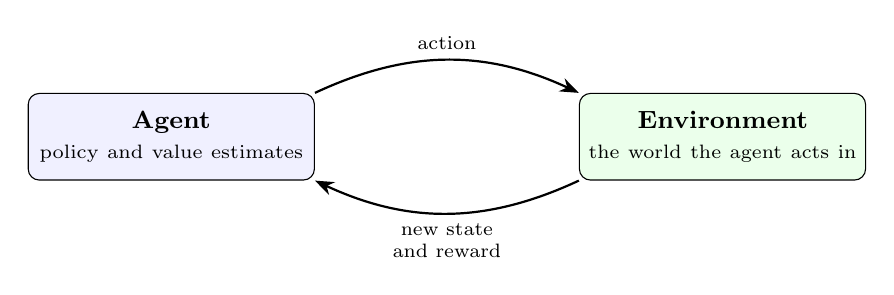
\begin{tikzpicture}[
    box/.style={draw, rounded corners, fill=blue!6, minimum height=1.1cm, text width=3.4cm, align=center, font=\small},
    arr/.style={-{Stealth[length=2.4mm]}, thick}]
\node[box] (agent) at (0,0) {\textbf{Agent}\\ \scriptsize policy and value estimates};
\node[box, fill=green!8] (env) at (7,0) {\textbf{Environment}\\ \scriptsize the world the agent acts in};
\draw[arr] (agent.north east) to[bend left=25] node[above, font=\scriptsize] {action} (env.north west);
\draw[arr] (env.south west) to[bend left=25] node[below, font=\scriptsize, align=center] {new state\\ and reward} (agent.south east);
\end{tikzpicture}
\caption{The reinforcement-learning loop: the agent acts, the environment answers with a new state and a reward, and the agent learns from the answer.}
\label{fig:loop}
\end{figure}

\textbf{Exploration versus exploitation.} An agent that only exploits repeats its first guesses and never discovers better options. An agent that only explores never uses what it has learned. Learning works only if the agent does both, usually exploring more at the beginning, when it knows little, and exploiting more later.

\textbf{Markov Decision Process.} This process is framed mathematically as a Markov Decision Process (MDP), in which future states depend only on the current state and action, not on the earlier sequence of events. In plain words, to decide what to do next the agent only needs to know where it is now, not how it got there. This is what makes a table of values, one entry per state and action, a sufficient memory in the maze.

\subsection{Types of reinforcement}

Two types of reinforcement are distinguished, borrowed from the psychology of behaviour (Table~\ref{tab:reinforcement}).

\begin{table}[H]
\centering
\small
\caption{Types of reinforcement.}
\label{tab:reinforcement}
\begin{tabularx}{\textwidth}{l X X X}
\toprule
Type & Definition & Advantages & Disadvantages \\
\midrule
Positive reinforcement & An event that occurs because of a behaviour increases the strength and frequency of that behaviour & Maximises performance; helps sustain change over time & Overuse can lead to excess states that reduce effectiveness \\
Negative reinforcement & A behaviour is strengthened because a negative condition is stopped or avoided & Increases how often the behaviour occurs; ensures a minimum standard of performance & May only encourage just enough action to avoid penalties \\
\bottomrule
\end{tabularx}
\end{table}

In the maze, the $+50$ for reaching the goal is positive reinforcement, and the penalties for steps and obstacles push the agent to avoid wasted moves and walls.

\subsection{Online and offline reinforcement learning}

RL can also be separated by \emph{how and when the agent gets its data} (Table~\ref{tab:onoff}). In \textbf{online RL} the agent learns by interacting with the environment in real time and collects fresh data as it goes. In \textbf{offline RL} (batch RL) the agent trains only on a static, pre-collected dataset, produced by other agents, human demonstrations or historical logs, and does not interact with the environment during learning.

\begin{table}[H]
\centering
\small
\caption{Online versus offline RL.}
\label{tab:onoff}
\begin{tabularx}{\textwidth}{l X X}
\toprule
Aspect & Online RL & Offline RL \\
\midrule
Data acquisition & Direct, real-time interaction with the environment & Static, pre-collected dataset \\
Adaptivity & High; adapts continuously & Limited; depends on dataset coverage \\
Suitability & When environment access or simulation is feasible & When interaction is costly or risky \\
Challenges & Resource-intensive, potentially unsafe & Distributional shift, counterfactual inference issues \\
\bottomrule
\end{tabularx}
\end{table}

The demonstration is online RL: the agent learns by acting in a simulated maze, where being ``unsafe'' costs nothing.

\subsection{Applications}

RL is applied in four main areas: \textbf{robotics} (automating tasks in structured environments such as manufacturing, where robots learn to optimise their movements), \textbf{games} (strategies for chess, Go and video games, in many cases outperforming human players), \textbf{industrial control} (real-time adjustment and optimisation, for example refining processes in the oil and gas industry) and \textbf{personalised training systems} (customising instructional content to each person's learning pattern).

\subsection{Advantages and limitations}

\begin{table}[H]
\centering
\small
\caption{Advantages and limitations of RL.}
\label{tab:proscons}
\begin{tabularx}{\textwidth}{X X}
\toprule
Advantages & Limitations \\
\midrule
Solves complex sequential decision problems where other approaches fail & Computationally intensive: needs large amounts of data and processing power \\
Learns from real-time interaction and adapts to changing environments & Reward design is critical; poor design leads to unintended behaviour \\
Needs no labelled data, unlike supervised learning & Not suitable for simple problems, where traditional methods are more efficient \\
Can discover strategies beyond human intuition & Hard to debug and interpret, so decisions are difficult to explain \\
Handles uncertainty and stochastic environments & The exploration--exploitation trade-off needs careful balancing \\
\bottomrule
\end{tabularx}
\end{table}

% =====================================================================
\section{How the Two Fit Together}
\label{sec:link}

Sections~\ref{sec:agents} and~\ref{sec:rl} use the same word, \emph{agent}, and describe the same cycle from two sides. The first describes what an agent \emph{is}: something that observes, reasons, plans, acts and refines itself. The second describes one way the last ability can be achieved: by learning from rewards. An \textbf{RL agent is an AI agent whose self-refinement comes from rewards}. Table~\ref{tab:mapping} shows the correspondence.

\begin{table}[H]
\centering
\small
\caption{Features of an AI agent and the matching elements of reinforcement learning.}
\label{tab:mapping}
\begin{tabularx}{\textwidth}{l X X}
\toprule
AI agent & Reinforcement learning & Maze demo (Section~\ref{sec:demo}) \\
\midrule
Observing & The agent observes the \textbf{state} & knows which cell it is in \\
Reasoning, planning & The \textbf{policy} maps states to actions; the \textbf{value function} judges long-term benefit & picks the move with the highest Q-value, sometimes a random one \\
Acting & The agent performs an \textbf{action} & moves left, right, up or down \\
Self-refining & The agent updates its policy and value function from the \textbf{reward} and the new state & updates its Q-table after every move \\
Memory & What the agent has learned is kept between attempts & the Q-table \\
Tools & The set of available actions & the four moves \\
Goal & Maximise cumulative reward & reach the exit with as few steps as possible \\
Collaborating & (outside the scope of a single RL agent) & not used \\
\bottomrule
\end{tabularx}
\end{table}

The relation is not symmetrical. Not every AI agent uses RL: an agent built on a language model, for example, may reason and use tools without being trained by rewards. And RL is a general learning method whose ``agent'' can be very simple. What the two share is the picture of an entity that acts in an environment to reach a goal and gets better through experience.

% =====================================================================
\section{Demonstration: A Q-learning Agent in a Maze}
\label{sec:demo}

This section implements a maze-crossing task as a small AI agent and measures what it learns. The full code and all outputs are in \code{notebook/agent\_rl\_demo.ipynb}.

\subsection{The environment}

The maze is a 10 $\times$ 10 grid in which each cell is a free path (0) or an obstacle (1). The agent starts at the top-left cell $(0,0)$ and has to reach the bottom-right cell $(9,9)$. In each cell it can try four actions: left, right, up, down. The layout in Figure~\ref{fig:maze} is my own; it has 59 free cells, 41 obstacles, and the shortest route from S to G, found with an ordinary breadth-first search only to have a true optimum to compare with, is \textbf{22 steps}.

\begin{figure}[H]
\centering
\includegraphics[width=0.45\textwidth]{maze.png}
\caption{The environment: S is the start, G the goal, dark cells are obstacles.}
\label{fig:maze}
\end{figure}

The rewards are fixed, and each has a purpose (Table~\ref{tab:rewards}).

\begin{table}[H]
\centering
\small
\caption{Rewards of the maze.}
\label{tab:rewards}
\begin{tabularx}{\textwidth}{l r X}
\toprule
Event & Reward & Purpose \\
\midrule
Reaching the goal & $+50$ & the outcome we want; large enough to outweigh the cost of the walk \\
Every ordinary step & $-1$ & a small cost for time; without it a long wandering path would be as good as a short one, so the agent would have no reason to find the \emph{shortest} path \\
Walking into an obstacle or off the grid & $-10$ & a strong penalty; the attempt (episode) ends \\
\bottomrule
\end{tabularx}
\end{table}

One \textbf{episode} is one attempt, from the start cell until the agent reaches the goal, crashes or runs out of moves (we allow at most 200). \textbf{Training} is many episodes in a row, during which the agent keeps what it has learned.

\subsection{Method: Q-learning}

\paragraph{The Q-table.} To act well, the agent has to know, for every cell and every move, \emph{how good that move is}, counting everything that follows it. Q-learning keeps these judgements in a table, a cheat sheet that fills itself in, with one row per cell and one column per action. Each entry, a \textbf{Q-value}, answers: ``if I make this move from this cell and then keep playing well, how much total reward can I expect?'' It is the value function of Section~\ref{sec:rl} for state--action pairs. The table starts at zero, because the agent initially knows nothing, and it is the agent's memory. Once the table is good, the policy is simple: \emph{in each cell, take the move with the highest Q-value.}

\paragraph{Exploration versus exploitation.} Think of choosing a restaurant: always returning to the first place you tried means you may never find a better one, while always trying somewhere new means you never enjoy the best place you know. The agent faces the same trade-off. It uses the standard \textbf{$\varepsilon$-greedy} rule: with probability $\varepsilon$ it makes a random move (explores), otherwise it takes its best known move (exploits). Here $\varepsilon$ starts at 0.5 and is multiplied by 0.995 after each episode, never going below 0.01: it explores a lot when it knows little and exploits more as its table becomes reliable.

\paragraph{The learning step.} After each move the agent asks two questions. \emph{What did I expect this move to be worth?} That is its current Q-value. \emph{What do I now believe it is worth?} That is the reward it just received plus the value of the best move from the cell it landed in, counted at 90\% (the \textbf{discount factor} $\gamma = 0.9$, because a later reward is a little less certain than one received now). The gap between the two is the agent's surprise, and the agent moves its Q-value 10\% of the way towards the new belief (the \textbf{learning rate} $\alpha = 0.1$). It takes only a small step because one experience may be a fluke; many small steps average out the luck. This is the standard Q-learning update rule, written in the notebook as:

\begin{codeblock}
def update(Q, s, a, r, s_next, done):
    expected = Q[s][a]
    believed = r if done else r + GAMMA * Q[s_next].max()   # GAMMA = 0.9
    Q[s][a] = expected + ALPHA * (believed - expected)        # ALPHA = 0.1
\end{codeblock}

A worked step from the notebook: the agent moves right from cell $(0,1)$ to $(0,2)$ and receives $-1$. It expected the move to be worth 0, but it already values the best move from $(0,2)$ at 6, so its new belief is $-1 + 0.9 \times 6 = 4.4$. The Q-value rises from 0 to $0.1 \times 4.4 = 0.44$. Repeated over thousands of moves, this is how the value of the goal \textbf{spreads backwards through the maze}: first the cells next to the goal become valuable, then the cells next to those, until the start.

\paragraph{Parameters.} The values used are listed in Table~\ref{tab:params}.

\begin{table}[H]
\centering
\small
\caption{Training parameters.}
\label{tab:params}
\begin{tabular}{l r l}
\toprule
Parameter & Value & Meaning \\
\midrule
Episodes & 5,000 & number of attempts \\
Learning rate $\alpha$ & 0.1 & how far each experience moves a Q-value \\
Discount factor $\gamma$ & 0.9 & weight of future rewards \\
Exploration $\varepsilon$ & 0.5 $\rightarrow$ 0.01 & starts at 0.5, $\times$ 0.995 per episode \\
Maximum moves per episode & 200 & an attempt is cut off after this \\
\bottomrule
\end{tabular}
\end{table}

\subsection{Baseline: an agent without knowledge}

Before learning, the agent's only option is a random move. This baseline shows how hard the task is: in 1,000 attempts a random agent \textbf{never} reached the goal, and its attempts lasted only 1.5 moves on average before it walked into a wall or off the grid. The first episodes of the learning agent look exactly like this.

\subsection{Training results}

Figure~\ref{fig:training} shows the 5,000 training episodes.

\begin{figure}[H]
\centering
\includegraphics[width=\textwidth]{training_curves.png}
\caption{Left: total reward per episode (grey) and its average over 100 episodes (blue). Middle: success rate. Right: exploration rate $\varepsilon$.}
\label{fig:training}
\end{figure}

The agent reached the goal for the first time in \textbf{episode 721}. In the last 500 episodes it succeeded \textbf{89\%} of the time with an average reward of 23.4. The curves show three things.

\begin{itemize}
    \item \textbf{The reward first falls, then rises.} For 720 episodes the agent never finds the exit, yet the average reward drops from about $-10$ to about $-30$. The agent learns the \emph{first} lesson before the second. Early attempts end in a crash after one or two moves ($-10$). Soon it learns that walls hurt and avoids them, but it does not yet know where the exit is, so it wanders safely along the corridors, paying $-1$ for every move until the 200-move limit. Longer attempts give a lower total. Only when the value of the goal reaches the start does the curve turn upward.
    \item \textbf{Success stops near 90\%, not 100\%.} While $\varepsilon$ is above its floor of 0.01 the agent still makes occasional random moves, and a random move next to a wall ends the attempt. The downward spikes of the grey line late in training are such episodes.
    \item \textbf{Success follows exploration.} $\varepsilon$ reaches its floor after about 780 episodes; the agent starts succeeding at about that time, and the success rate keeps rising as the agent explores less and trusts its table more.
\end{itemize}

\subsection{What the agent learned}

To see what the agent has learned, it is made to act \emph{greedily} from the start, always taking the best move in its Q-table and never exploring. It reaches the goal in \textbf{22 steps with a total reward of 29}: the shortest possible route, found from rewards alone (Figure~\ref{fig:path}). The reward is $50 - 21 = 29$: the prize minus one point for each of the 21 ordinary steps before the final move.

\begin{figure}[H]
\centering
\begin{subfigure}{0.46\textwidth}\includegraphics[width=\linewidth]{learned_path.png}\caption{The learned path: 22 steps.}\end{subfigure}\hfill
\begin{subfigure}{0.52\textwidth}\includegraphics[width=\linewidth]{policy.png}\caption{The learned policy and the value of each cell.}\end{subfigure}
\caption{What the trained agent has learned.}
\label{fig:path}
\end{figure}

The right-hand picture shows the whole policy: the best move in every free cell as an arrow, and the highest Q-value of the cell as colour. Three things stand out.
\begin{itemize}
    \item \textbf{Values grow towards the goal.} A cell close to G is worth more than a cell far away, because fewer step penalties remain and the prize is discounted less.
    \item \textbf{Cells off the route are poorly learned.} In the top row, the arrows of cells $(0,6)$ and $(0,7)$ point at each other: an agent placed there would walk back and forth forever. The agent always started at S during training, so it gained experience mainly along the routes it used from there.
    \item \textbf{G itself is pale.} The attempt ends at G, so no move is ever made \emph{from} it; the value belongs to the move \emph{into} G, which is why the cell next to it, $(8,9)$, is the darkest.
\end{itemize}

\subsection{Random agent versus trained agent}

The two agents were compared over 100 runs from the start cell. Because the trained agent behaves the same way every time from S, it was also tested from \textbf{every free cell} of the maze (58 starting points): a policy that has really learned the maze should reach the goal from anywhere, not only from where it practised.

\begin{table}[H]
\centering
\small
\caption{Random agent versus trained agent.}
\label{tab:compare}
\begin{tabular}{l r r r}
\toprule
 & Reached the goal & Average steps (successes) & Average reward \\
\midrule
Random agent, from S (100 runs) & 0\% & -- & $-10.6$ \\
Trained agent, from S (100 runs) & 100\% & 22.0 & 29.0 \\
Trained agent, from every free cell (58 starts) & 47\% & 11.7 & $-82.1$ \\
\bottomrule
\end{tabular}
\end{table}

\begin{figure}[H]
\centering
\includegraphics[width=0.6\textwidth]{comparison.png}
\caption{Share of runs that reach the goal.}
\label{fig:compare}
\end{figure}

The first two rows give the main result. With the same maze, the same four moves and the same rules, the agent without knowledge never reaches the goal, while the agent that learned from 5,000 attempts reaches it every time from the start, along the shortest route.

The third row is less good. Started from the other cells, the trained agent reaches the goal from only 27 of 58 cells (47\%). From 29 cells it does not crash but \textbf{loops}: it moves back and forth between two cells until the 200-move limit, which explains the very low average reward (about $-1$ for each wasted move); from the remaining 2 cells it walks into a wall. In a cell far from its practised routes, the Q-values come from a few bad experiences, and two neighbouring cells can each rate ``go to the other one'' as best. Nothing in the reward signal ever corrected this, because the agent never started there.

I do not think this is a bug in the code. It follows from learning by experience: the agent is only as good as the situations it has practised. It also shows why evaluating a learner only under the conditions it trained on (the first two rows) can be misleading. A way to improve it would be to start training episodes from random cells, so that every part of the maze is experienced; this was not done here, to keep the setup simple.

% =====================================================================
\section{Discussion and Conclusion}
\label{sec:disc}

\subsection{Limitations of the approach}

The maze is small on purpose, so every part of the agent can be inspected. Even so, the main limitations of AI agents and of RL all appear in it.

\begin{itemize}
    \item \textbf{Reward design decides behaviour.} The $-1$ per step is what makes the agent look for the \emph{shortest} path; without it any path to the goal would be equally good. A badly chosen reward would make the agent learn the wrong thing.
    \item \textbf{Exploration and exploitation must be balanced.} Too little exploration locks the agent into its first route; too much keeps it crashing. The decay schedule of $\varepsilon$ is a design choice, not something the agent learns.
    \item \textbf{Learning is computationally expensive,} and so is building agents. In this 10 $\times$ 10 grid with four moves the agent failed 720 times before it reached the goal once, and it used 5,000 episodes to become reliable. A table with one row per state does not scale to real robots or games, which have far too many states.
    \item \textbf{The agent knows only what it has experienced.} Started anywhere but S, it reaches the goal only about half the time.
    \item \textbf{It is hard to explain.} The policy is readable here because it is a small table of arrows, but a decision made by a larger learned model is much harder to justify.
    \item \textbf{Trial and error is risky.} High ethical stakes and unpredictable physical settings, such as surgery or disaster response, are poor fits for agents. Failing hundreds of times is fine in a simulation but not on a real road or in an operating room. Where interaction is costly or risky, offline RL on recorded data is an option, though it has its own problem of dataset coverage.
\end{itemize}

\subsection{Conclusion}

An AI agent is a goal-driven system that observes, reasons, plans, acts and refines itself, with a persona, memory, tools and a model behind it. Reinforcement learning is a way for an agent to refine itself by trial and error, guided only by rewards, balancing exploration and exploitation. In the demonstration, a Q-learning agent that started with no knowledge went from never reaching the exit to reaching it every time from the start, by the shortest route of 22 steps, using only the rewards $+50$, $-1$ and $-10$. It also showed a limit: from other starting cells the learned policy often fails, because the agent had never practised there.

Three extensions were left out: starting training from random cells to remove the loops, a larger maze where a neural network has to replace the table, and several agents in one environment (the multi-agent case).

% =====================================================================


\end{document}
